\documentclass[aspectratio=169,11pt]{beamer}

\usepackage[utf8]{inputenc}
\usepackage[T1]{fontenc}
\usepackage[spanish,es-nodecimaldot]{babel}
\usepackage{lmodern}
\usepackage{amsmath,amssymb,bm}
\usepackage{booktabs,array,multirow}
\usepackage{graphicx}
\usepackage{tikz}
\usetikzlibrary{positioning}
\usepackage{listings}
\usepackage{xcolor}
\usepackage{hyperref}

\usetheme{Madrid}
\usecolortheme{default}
\setbeamertemplate{navigation symbols}{}
\setbeamertemplate{footline}[frame number]

\definecolor{MainBlue}{RGB}{26,74,122}
\definecolor{SoftBlue}{RGB}{230,240,250}
\definecolor{SoftGray}{RGB}{245,245,245}
\definecolor{DeepRed}{RGB}{154,42,42}
\definecolor{DarkGreen}{RGB}{34,102,68}

\setbeamercolor{title}{fg=MainBlue}
\setbeamercolor{frametitle}{fg=white,bg=MainBlue}
\setbeamercolor{structure}{fg=MainBlue}
\setbeamercolor{block title}{bg=MainBlue!12, fg=black}
\setbeamercolor{block body}{bg=SoftGray, fg=black}
\setbeamercolor{alerted text}{fg=DeepRed}

\graphicspath{{figures/}}

\lstset{
  language=Python,
  basicstyle=\ttfamily\scriptsize,
  keywordstyle=\color{MainBlue}\bfseries,
  commentstyle=\color{DarkGreen},
  showstringspaces=false,
  frame=single,
  backgroundcolor=\color{SoftGray},
  breaklines=true,
  columns=fullflexible
}

\title{C\'omo escribir el informe del curso}
\subtitle{Gu\'ia para informes manuscritos}
\author{Modelos Computacionales para F\'isica y Astronom\'ia}
\date{\today}

\begin{document}

\begin{frame}[plain]
\vfill
\centering
{\color{MainBlue}\Huge\bfseries C\'omo escribir el informe del curso\par}
\vspace{0.35cm}
{\Large Gu\'ia para informes manuscritos\par}
\vspace{0.6cm}
{\large Modelos Computacionales para F\'isica y Astronom\'ia\par}
\vspace{0.2cm}
{\normalsize \today\par}
\vfill
\end{frame}

\begin{frame}
\frametitle{Objetivo de la clase}
\begin{block}{Meta principal}
Que cada estudiante salga de esta clase sabiendo \alert{c\'omo transformar un enunciado computacional en un informe claro, breve y defendible}.
\end{block}

\vspace{0.2cm}
\begin{itemize}
    \item Qu\'e debe tener una \textbf{introducci\'on}.
    \item C\'omo construir un \textbf{marco te\'orico} sin copiar el enunciado.
    \item C\'omo separar \textbf{metodolog\'ia, resultados, an\'alisis y conclusiones}.
    \item C\'omo citar \textbf{bibliograf\'ia} y material del curso.
    \item C\'omo organizar un informe cuando hay \textbf{2 o 3 problemas}.
\end{itemize}
\end{frame}

\begin{frame}
\frametitle{Ruta sugerida para 90 minutos}
\begin{columns}[T]
\begin{column}{0.48\textwidth}
\begin{block}{Primera mitad}
\begin{itemize}
    \item Estructura general del informe.
    \item Introducci\'on y marco te\'orico.
    \item Metodolog\'ia y tratamiento del c\'odigo.
\end{itemize}
\end{block}
\end{column}
\begin{column}{0.48\textwidth}
\begin{block}{Segunda mitad}
\begin{itemize}
    \item Resultados vs. an\'alisis.
    \item Conclusiones y bibliograf\'ia.
    \item Ejemplo completo con 2 problemas.
\end{itemize}
\end{block}
\end{column}
\end{columns}

\vspace{0.25cm}
\begin{alertblock}{Regla de oro}
El informe \textbf{no es el cuaderno de c\'odigo} ni una copia del enunciado: es una explicaci\'on razonada de lo que se hizo, por qu\'e se hizo y qu\'e se concluye.
\end{alertblock}
\end{frame}

\begin{frame}
\frametitle{\textquestiondown{}Para qu\'e sirve realmente el informe?}
\begin{itemize}
    \item Mostrar que el estudiante \textbf{entendi\'o el problema}.
    \item Justificar el \textbf{modelo matem\'atico} y el \textbf{m\'etodo num\'erico} usado.
    \item Presentar evidencia: figuras, tablas, valores relevantes, tendencias.
    \item Interpretar los resultados: \textbf{no basta con graficar}.
    \item Comunicar con orden y precisi\'on, como en un mini-art\'iculo cient\'ifico.
\end{itemize}

\vspace{0.2cm}
\begin{block}{Lo que normalmente se eval\'ua}
Claridad, correcci\'on conceptual, calidad del an\'alisis, uso razonable de resultados computacionales y presentaci\'on general.
\end{block}
\end{frame}

\begin{frame}
\frametitle{Estructura m\'inima recomendada}
\begin{center}
\begin{tikzpicture}[node distance=0.65cm, every node/.style={rounded corners=2pt, align=center}]
\node[draw, fill=SoftBlue, minimum width=2.2cm, minimum height=0.9cm] (a) {Introducci\'on};
\node[draw, fill=SoftBlue, minimum width=2.4cm, minimum height=0.9cm, right=0.35cm of a] (b) {Marco\\te\'orico};
\node[draw, fill=SoftBlue, minimum width=2.6cm, minimum height=0.9cm, right=0.35cm of b] (c) {Metodolog\'ia};
\node[draw, fill=SoftBlue, minimum width=2.2cm, minimum height=0.9cm, right=0.35cm of c] (d) {Resultados};
\node[draw, fill=SoftBlue, minimum width=2.2cm, minimum height=0.9cm, below=0.6cm of c] (e) {An\'alisis};
\node[draw, fill=SoftBlue, minimum width=2.3cm, minimum height=0.9cm, left=0.35cm of e] (f) {Conclusiones};
\node[draw, fill=SoftBlue, minimum width=2.4cm, minimum height=0.9cm, right=0.35cm of e] (g) {Bibliograf\'ia};
\draw[-latex, thick, MainBlue] (a) -- (b);
\draw[-latex, thick, MainBlue] (b) -- (c);
\draw[-latex, thick, MainBlue] (c) -- (d);
\draw[-latex, thick, MainBlue] (d) -- (e);
\draw[-latex, thick, MainBlue] (e) -- (f);
\draw[-latex, thick, MainBlue] (e) -- (g);
\end{tikzpicture}
\end{center}

\vspace{0.2cm}
\begin{alertblock}{Idea clave}
Cada secci\'on responde una pregunta distinta: \textbf{qu\'e problema}, \textbf{con qu\'e herramientas}, \textbf{qu\'e obtuve}, \textbf{qu\'e significa} y \textbf{qu\'e concluyo}.
\end{alertblock}
\end{frame}

\begin{frame}
\frametitle{\textquestiondown{}Qu\'e es una buena introducci\'on?}
\begin{columns}[T]
\begin{column}{0.55\textwidth}
\begin{block}{La introducci\'on debe}
\begin{itemize}
    \item presentar el tema general,
    \item explicar el problema que se estudiar\'a,
    \item indicar el objetivo del trabajo,
    \item anticipar brevemente el enfoque computacional.
\end{itemize}
\end{block}
\end{column}
\begin{column}{0.42\textwidth}
\begin{block}{Evitar}
\begin{itemize}
    \item copiar el enunciado,
    \item empezar con ecuaciones sin contexto,
    \item contar paso a paso el c\'odigo.
\end{itemize}
\end{block}
\end{column}
\end{columns}

\vspace{0.25cm}
\begin{alertblock}{Plantilla simple}
``En este informe se estudia [...]. El objetivo es [...]. Para ello se utiliza [...]. Finalmente, se analizan [...].''
\end{alertblock}
\end{frame}

\begin{frame}
\frametitle{Ejemplo breve de introducci\'on}
\small
\begin{block}{Ejemplo de redacci\'on}
En este informe se estudian dos sistemas din\'amicos mediante herramientas computacionales: el mapa de H\'enon y un modelo SIR con vacunaci\'on. El objetivo es comparar c\'omo reglas matem\'aticas relativamente simples pueden producir comportamientos complejos y visualizaciones informativas. Para ello se implementan algoritmos num\'ericos en Python, se generan trayectorias y se analizan figuras representativas. Finalmente, se discuten las principales diferencias entre un sistema discreto ca\'otico y un sistema continuo de ecuaciones diferenciales.
\end{block}

\vspace{0.2cm}
\begin{alertblock}{Observaci\'on}
La introducci\'on \textbf{no demuestra} resultados: s\'olo instala el problema, el objetivo y el plan del informe.
\end{alertblock}
\end{frame}

\begin{frame}
\frametitle{\textquestiondown{}Qu\'e es el marco te\'orico?}
\begin{itemize}
    \item Es la secci\'on donde se presentan las \textbf{ideas, conceptos y ecuaciones} que permiten entender el problema.
    \item Debe ser \textbf{selectivo}: s\'olo lo necesario para comprender el desarrollo posterior.
    \item Puede incluir definiciones, variables, par\'ametros, unidades, interpretaci\'on f\'isica y referencias.
\end{itemize}

\vspace{0.2cm}
\begin{block}{Ejemplo de contenidos de marco te\'orico}
\begin{itemize}
    \item Para H\'enon: sistema din\'amico discreto, sensibilidad a condiciones iniciales, atractor.
    \item Para SIR: significado de $S$, $I$, $R$, tasas $\beta$, $\gamma$, $v$ y rol de la vacunaci\'on.
\end{itemize}
\end{block}
\end{frame}

\begin{frame}
\frametitle{Marco te\'orico: qu\'e s\'i y qu\'e no}
\begin{columns}[T]
\begin{column}{0.48\textwidth}
\begin{block}{S\'i}
\begin{itemize}
    \item Ecuaciones importantes.
    \item Significado de variables.
    \item Contexto cient\'ifico breve.
    \item Referencias a apuntes o libros.
\end{itemize}
\end{block}
\end{column}
\begin{column}{0.48\textwidth}
\begin{block}{No}
\begin{itemize}
    \item Derivaciones largu\'isimas si no fueron pedidas.
    \item P\'aginas de teor\'ia que luego no se usan.
    \item Definiciones sin explicar para qu\'e sirven.
\end{itemize}
\end{block}
\end{column}
\end{columns}

\vspace{0.2cm}
\begin{alertblock}{Criterio pr\'actico}
Si una ecuaci\'on o concepto no vuelve a aparecer en la metodolog\'ia, resultados o an\'alisis, probablemente sobra.
\end{alertblock}
\end{frame}

\begin{frame}
\frametitle{Metodolog\'ia: explicar el proceso}
\begin{block}{Aqu\'i se responde: \textit{\textquestiondown{}c\'omo se resolvi\'o el problema?}}
\begin{itemize}
    \item modelo o ecuaciones utilizadas,
    \item algoritmo num\'erico,
    \item par\'ametros y condiciones iniciales,
    \item criterios de simulaci\'on,
    \item qu\'e se grafic\'o o compar\'o.
\end{itemize}
\end{block}

\vspace{0.2cm}
\begin{alertblock}{Importante}
En un informe manuscrito, la metodolog\'ia debe \textbf{describir el procedimiento}, no pegar 3 p\'aginas de c\'odigo.
\end{alertblock}
\end{frame}

\begin{frame}[fragile]{\textquestiondown{}Cu\'anto c\'odigo conviene mostrar?}
\begin{columns}[T]
\begin{column}{0.53\textwidth}
\begin{block}{Regla recomendada}
\begin{itemize}
    \item incluir s\'olo \textbf{fragmentos peque\~nos} si ayudan a explicar la idea,
    \item resumir el resto en palabras,
    \item si el curso no pide anexos, el c\'odigo completo \textbf{no reemplaza} el informe.
\end{itemize}
\end{block}
\end{column}
\begin{column}{0.43\textwidth}
\begin{lstlisting}
for n in range(10000):
    x_new = 1 - a*x**2 + y
    y_new = b*x
    x, y = x_new, y_new
\end{lstlisting}
\end{column}
\end{columns}

\vspace{0.15cm}
\begin{alertblock}{C\'omo comentarlo en el informe}
``Se iter\'o el mapa durante 10\,000 pasos, descartando los primeros 1\,000 transitorios, para visualizar el atractor en el plano $(x,y)$.''
\end{alertblock}
\end{frame}

\begin{frame}
\frametitle{Resultados \textbf{no} son an\'alisis}
\begin{columns}[T]
\begin{column}{0.48\textwidth}
\begin{block}{Resultados}
\begin{itemize}
    \item figuras,
    \item tablas,
    \item valores medidos,
    \item observaciones directas.
\end{itemize}
\end{block}
\end{column}
\begin{column}{0.48\textwidth}
\begin{block}{An\'alisis / discusi\'on}
\begin{itemize}
    \item interpretaci\'on,
    \item comparaci\'on con teor\'ia,
    \item limitaciones,
    \item explicaci\'on del comportamiento observado.
\end{itemize}
\end{block}
\end{column}
\end{columns}

\vspace{0.2cm}
\begin{alertblock}{Ejemplo}
``La curva de $I(t)$ alcanza un m\'aximo cercano a 0.17'' es resultado.\newline
``Ese m\'aximo disminuye por efecto de la vacunaci\'on, lo que reduce el n\'umero de susceptibles'' es an\'alisis.
\end{alertblock}
\end{frame}

\begin{frame}
\frametitle{C\'omo presentar resultados}
\begin{itemize}
    \item Cada figura debe tener un \textbf{prop\'osito claro}.
    \item El texto debe decir \textbf{qu\'e mirar} en esa figura.
    \item No llenar el informe con gr\'aficos repetidos.
    \item Si hay muchas simulaciones, elegir las m\'as informativas.
\end{itemize}

\vspace{0.2cm}
\begin{block}{Frase \'util}
``La Figura X muestra [...]. Se observa que [...]. Esto sugiere que [...].''
\end{block}

\vspace{0.2cm}
\begin{alertblock}{Manuscrito}
Si el informe es a mano, pueden pegar o dibujar esquem\'aticamente las figuras principales, pero el comentario anal\'itico debe quedar escrito con claridad.
\end{alertblock}
\end{frame}

\begin{frame}
\frametitle{\textquestiondown{}Qu\'e va en las conclusiones?}
\begin{itemize}
    \item Responder si se cumpli\'o el objetivo planteado.
    \item Resumir los hallazgos principales en pocas ideas fuertes.
    \item Mencionar limitaciones o posibles extensiones si aporta valor.
\end{itemize}

\vspace{0.2cm}
\begin{block}{No hacer}
\begin{itemize}
    \item repetir todo el informe,
    \item introducir resultados nuevos,
    \item cerrar con frases vac\'ias como ``se hizo lo pedido y se obtuvo el gr\'afico''.
\end{itemize}
\end{block}
\end{frame}

\begin{frame}
\frametitle{Bibliograf\'ia y c\'omo citar}
\begin{columns}[T]
\begin{column}{0.52\textwidth}
\begin{block}{Cita en el texto}
\begin{itemize}
    \item ``Seg\'un Newman [1], ...''
    \item ``Como se discute en los apuntes del curso [2], ...''
\end{itemize}
\end{block}

\begin{block}{Lista final de referencias}
\small
[1] M. Newman, \textit{Computational Physics}, CreateSpace, 2013.\\[0.1cm]
[2] J. Peralta, \textit{Apuntes del curso}, 2025.
\end{block}
\end{column}
\begin{column}{0.43\textwidth}
\begin{alertblock}{Regla pr\'actica}
Si una idea, definici\'on, ecuaci\'on o algoritmo viene de una fuente externa, \textbf{debe citarse}.\newline
\newline
Si es desarrollo propio, no hace falta inventar una cita.
\end{alertblock}
\end{column}
\end{columns}
\end{frame}

\begin{frame}
\frametitle{Si el informe es manuscrito}
\begin{itemize}
    \item Mantener t\'itulos y subt\'itulos visibles.
    \item Escribir ecuaciones con notaci\'on consistente.
    \item Numerar figuras si las incluyen.
    \item Cuidar el orden visual: m\'argenes, separaci\'on y legibilidad.
\end{itemize}

\vspace{0.2cm}
\begin{block}{L\'imite de extensi\'on}
\textbf{No deber\'ia exceder 12 hojas.}
\end{block}

\vspace{0.1cm}
\begin{table}
\centering
\small
\begin{tabular}{>{\raggedright\arraybackslash}p{0.47\textwidth}c}
\toprule
Secci\'on & Hojas sugeridas \\
\midrule
Introducci\'on + marco te\'orico & 2--3 \\
Metodolog\'ia & 1--2 \\
Resultados + an\'alisis de cada problema & 5--6 \\
Conclusiones + bibliograf\'ia & 1--2 \\
\bottomrule
\end{tabular}
\end{table}
\end{frame}

\begin{frame}
\frametitle{\textquestiondown{}Separar o unir si hay 2 o 3 problemas?}
\begin{columns}[T]
\begin{column}{0.48\textwidth}
\begin{block}{Separar por problema}
Conviene si los problemas son \textbf{muy distintos} en modelo, m\'etodo o interpretaci\'on.
\end{block}
\end{column}
\begin{column}{0.48\textwidth}
\begin{block}{Unir en un solo relato}
Conviene si comparten una pregunta general, una metodolog\'ia o una comparaci\'on natural.
\end{block}
\end{column}
\end{columns}

\vspace{0.2cm}
\begin{alertblock}{Respuesta corta}
\textbf{Las dos opciones son v\'alidas}. Lo importante es que el informe se lea con l\'ogica y no como fragmentos pegados sin conexi\'on.
\end{alertblock}
\end{frame}

\begin{frame}
\frametitle{Dos estructuras posibles}
\small
\begin{columns}[T]
\begin{column}{0.48\textwidth}
\begin{block}{Opci\'on A: totalmente separada}
Introducci\'on general\\
Problema 1: teor\'ia, m\'etodo, resultados, an\'alisis\\
Problema 2: teor\'ia, m\'etodo, resultados, an\'alisis\\
Conclusiones generales
\end{block}
\end{column}
\begin{column}{0.48\textwidth}
\begin{block}{Opci\'on B: integrada}
Introducci\'on general\\
Marco te\'orico com\'un\\
Metodolog\'ia com\'un\\
Resultados y an\'alisis: problema 1\\
Resultados y an\'alisis: problema 2\\
Conclusiones comparativas
\end{block}
\end{column}
\end{columns}

\vspace{0.15cm}
\begin{alertblock}{Recomendaci\'on}
Para ahorrar espacio en un manuscrito de 12 hojas, la opci\'on \textbf{integrada} suele funcionar mejor cuando no conviene repetir teor\'ia o descripci\'on del procedimiento.
\end{alertblock}
\end{frame}

\begin{frame}
\frametitle{Ejemplo de caso con 2 problemas}
\begin{block}{Tomaremos dos ejercicios de una prueba antigua}
\begin{itemize}
    \item \textbf{Problema 1:} mapa de H\'enon, un sistema din\'amico discreto con atractor ca\'otico.
    \item \textbf{Problema 2:} modelo SIR con vacunaci\'on, resuelto con Runge--Kutta de cuarto orden.
\end{itemize}
\end{block}

\vspace{0.15cm}
\begin{alertblock}{Idea del ejemplo}
Aunque son temas distintos, ambos pueden presentarse bajo una misma idea: \textit{uso de herramientas computacionales para estudiar sistemas din\'amicos y visualizar su comportamiento}.\end{alertblock}
\end{frame}

\begin{frame}
\frametitle{Ejemplo de estructura integrada para esos 2 problemas}
\small
\begin{enumerate}
    \item \textbf{Introducci\'on:} motivaci\'on general sobre sistemas din\'amicos y simulaci\'on computacional.
    \item \textbf{Marco te\'orico:} diferencia entre sistemas discretos y continuos; nociones de atractor, variables epidemiol\'ogicas y par\'ametros.
    \item \textbf{Metodolog\'ia:} implementaci\'on en Python, selecci\'on de par\'ametros, generaci\'on de gr\'aficos.
    \item \textbf{Problema 1:} resultados del mapa de H\'enon y breve discusi\'on del caos.
    \item \textbf{Problema 2:} resultados del modelo SIR y discusi\'on del efecto de la vacunaci\'on.
    \item \textbf{Conclusiones:} contraste entre ambos tipos de din\'amica y valor de la simulaci\'on num\'erica.
\end{enumerate}
\end{frame}

\begin{frame}
\frametitle{Ejemplo de marco te\'orico compartido}
\small
\begin{columns}[T]
\begin{column}{0.48\textwidth}
\begin{block}{Mapa de H\'enon}
\[
 x_{n+1}=1-a x_n^2+y_n,
 \qquad y_{n+1}=b x_n.
\]
Sistema discreto donde interesa la estructura del atractor y la sensibilidad de la trayectoria.
\end{block}
\end{column}
\begin{column}{0.48\textwidth}
\begin{block}{Modelo SIR con vacunaci\'on}
\[
\frac{dS}{dt}=-\beta SI-vS,
\quad
\frac{dI}{dt}=\beta SI-\gamma I,
\quad
\frac{dR}{dt}=\gamma I+vS.
\]
Sistema continuo donde interesa la evoluci\'on temporal y el rol de los par\'ametros.
\end{block}
\end{column}
\end{columns}

\vspace{0.15cm}
\begin{alertblock}{Comentario}
Obs\'ervese que el marco te\'orico es breve: s\'olo deja instaladas las ecuaciones y la interpretaci\'on b\'asica necesaria.
\end{alertblock}
\end{frame}

\begin{frame}
\frametitle{Ejemplo de metodolog\'ia compartida}
\small
\begin{itemize}
    \item Se implementaron ambos problemas en Python.
    \item Para H\'enon se realizaron 10\,000 iteraciones, descartando 1\,000 transitorios.
    \item Para SIR se us\'o RK4 con par\'ametros $\beta=0.3$, $\gamma=0.1$, $v=0.05$ e integraci\'on entre 0 y 160 d\'ias.
    \item En ambos casos se construyeron figuras orientadas al an\'alisis: atractor, series temporales y diagrama de fase.
\end{itemize}

\vspace{0.2cm}
\begin{block}{Redacci\'on adecuada}
No hace falta copiar el script completo. Basta explicar el algoritmo, los par\'ametros elegidos y la finalidad de cada visualizaci\'on.
\end{block}
\end{frame}

\begin{frame}
\frametitle{Ejemplo de resultados: Problema 1}
\begin{columns}[T]
\begin{column}{0.54\textwidth}
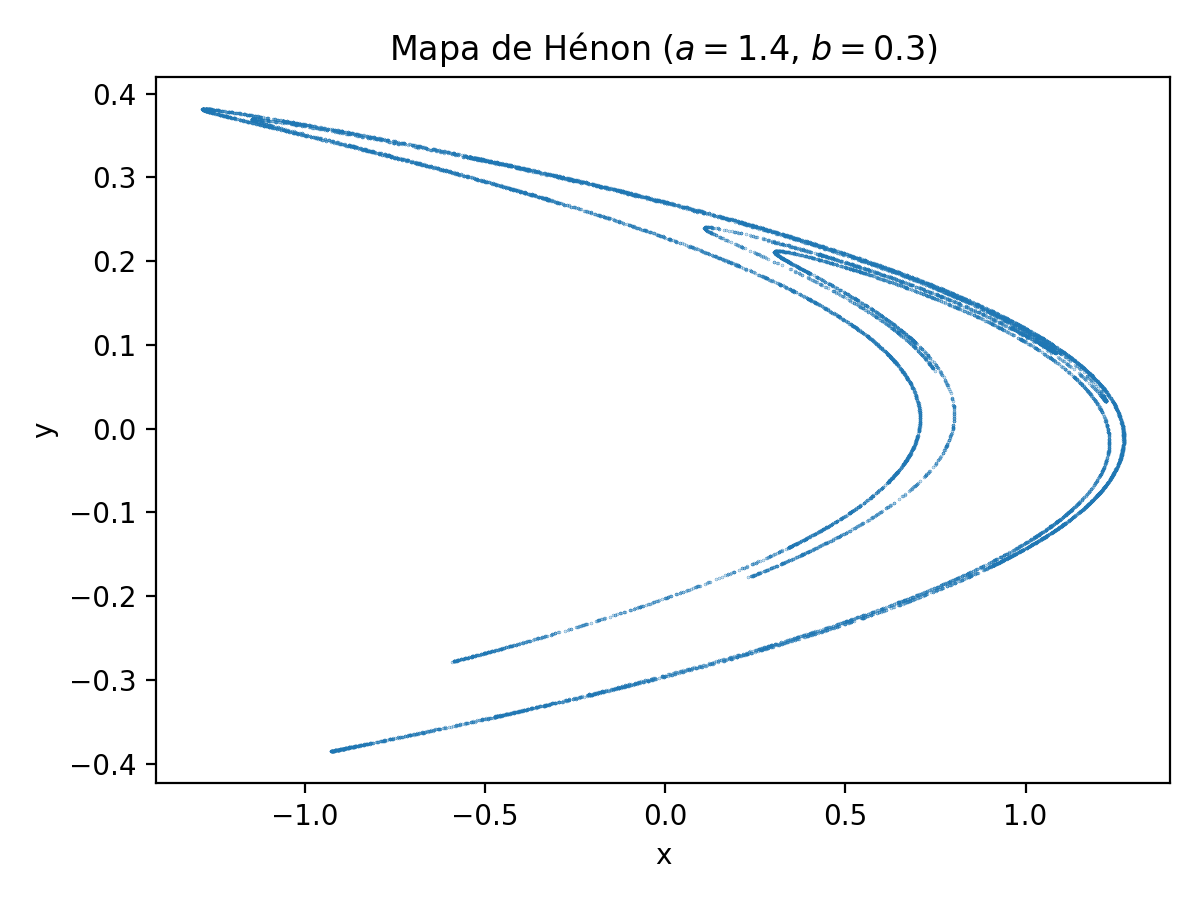
\includegraphics[width=\linewidth]{henon_attractor.png}
\end{column}
\begin{column}{0.42\textwidth}
\begin{block}{Texto posible en el informe}
La figura muestra la nube de puntos obtenida al iterar el mapa de H\'enon. Se observa una estructura no trivial y altamente plegada, compatible con un atractor extra\~no.
\end{block}
\end{column}
\end{columns}
\end{frame}

\begin{frame}
\frametitle{Ejemplo de an\'alisis: Problema 1}
\begin{block}{Interpretaci\'on}
La geometr\'ia del atractor indica que el sistema no converge a un punto fijo simple ni a una \'orbita peri\'odica elemental. La estructura observada sugiere comportamiento ca\'otico y dependencia sensible de las condiciones iniciales. El uso de muchas iteraciones y el descarte del transitorio permiten ver el r\'egimen asint\'otico con mayor claridad.
\end{block}

\vspace{0.2cm}
\begin{alertblock}{Observaci\'on did\'actica}
Primero se muestra \textbf{qu\'e aparece}. Despu\'es se explica \textbf{qu\'e significa}. Esa separaci\'on mejora mucho la calidad del informe.
\end{alertblock}
\end{frame}

\begin{frame}
\frametitle{Ejemplo de resultados: Problema 2}
\begin{columns}[T]
\begin{column}{0.56\textwidth}
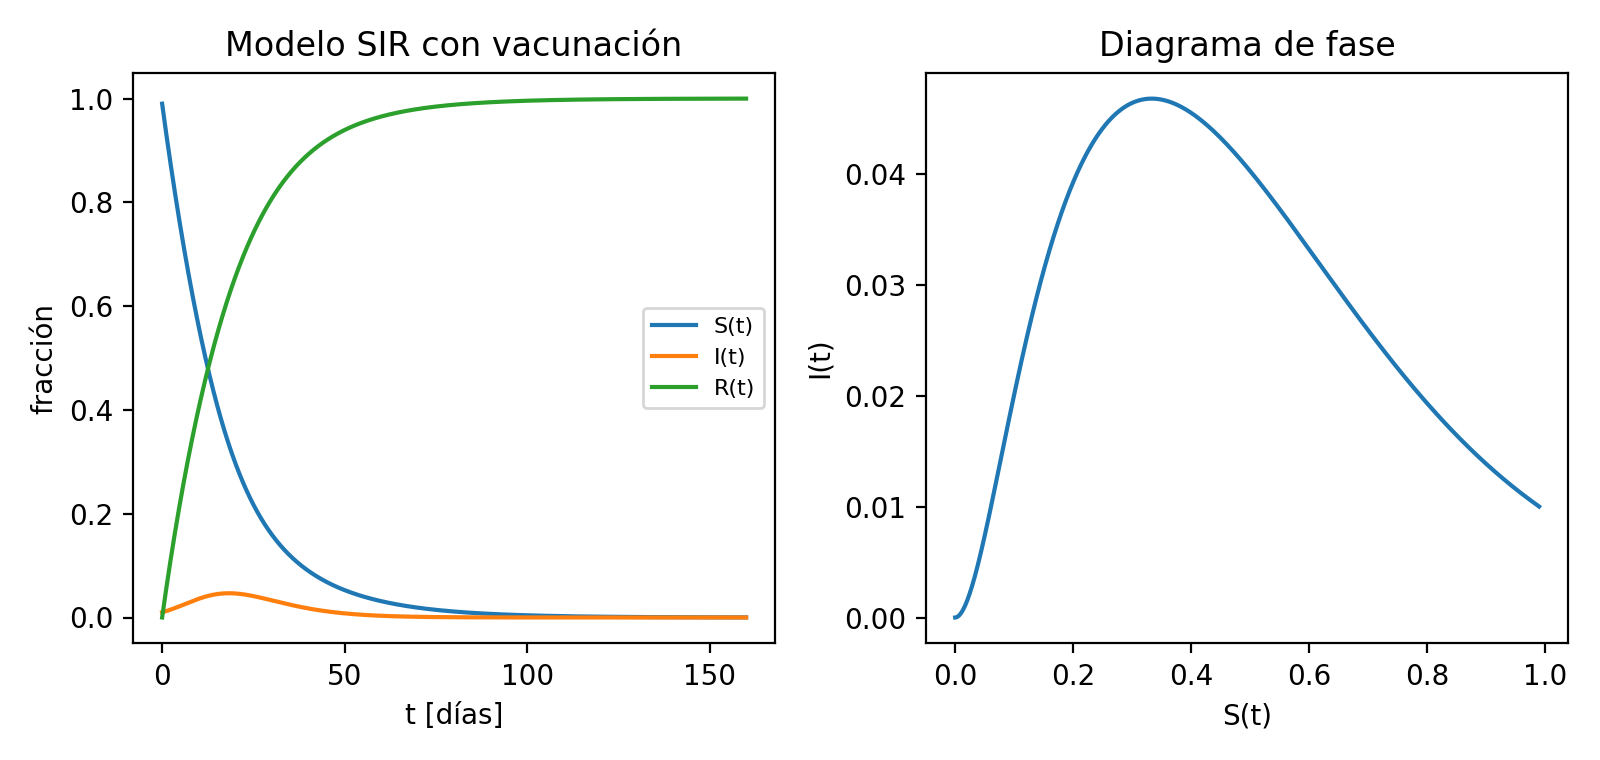
\includegraphics[width=\linewidth]{sir_vaccination.png}
\end{column}
\begin{column}{0.39\textwidth}
\begin{block}{Texto posible en el informe}
Las curvas muestran la disminuci\'on de susceptibles, el crecimiento y posterior ca\'ida de infectados, y el aumento de recuperados/vacunados. El diagrama de fase resume la trayectoria del sistema en el plano $(S,I)$.
\end{block}
\end{column}
\end{columns}
\end{frame}

\begin{frame}
\frametitle{Ejemplo de an\'alisis: Problema 2}
\begin{block}{Interpretaci\'on}
La vacunaci\'on act\'ua reduciendo la fracci\'on susceptible disponible para la infecci\'on. Como consecuencia, el m\'aximo de infectados disminuye y la epidemia se extingue m\'as r\'apidamente que en un escenario sin vacunaci\'on. El diagrama de fase permite ver esta transici\'on de forma compacta.
\end{block}

\vspace{0.2cm}
\begin{alertblock}{Otra vez: resultado vs. an\'alisis}
La figura es el resultado; la explicaci\'on epidemiol\'ogica de lo observado es el an\'alisis.
\end{alertblock}
\end{frame}

\begin{frame}
\frametitle{Ejemplo de conclusiones globales para 2 problemas}
\small
\begin{block}{Modelo de cierre}
Los dos problemas estudiados muestran c\'omo la simulaci\'on computacional permite analizar sistemas din\'amicos de naturaleza distinta. En el mapa de H\'enon se observ\'o una estructura compatible con caos y atractores extra\~nos. En el modelo SIR con vacunaci\'on se vio que la modificaci\'on de par\'ametros tiene consecuencias directas sobre la evoluci\'on de la poblaci\'on infectada. En conjunto, ambos ejercicios ilustran el valor de combinar modelo matem\'atico, implementaci\'on num\'erica y an\'alisis cr\'itico de figuras.
\end{block}
\end{frame}

\begin{frame}
\frametitle{Errores frecuentes que bajan mucho la nota}
\begin{itemize}
    \item Copiar el enunciado como si fuera introducci\'on.
    \item Poner ecuaciones sin explicar variables ni par\'ametros.
    \item Mostrar gr\'aficos sin comentarlos.
    \item Mezclar resultados y conclusiones en un solo bloque confuso.
    \item Llenar el informe con c\'odigo en vez de describir el procedimiento.
    \item No citar apuntes, libros o referencias usadas.
    \item Entregar un manuscrito desordenado o demasiado extenso.
\end{itemize}
\end{frame}

\begin{frame}
\frametitle{Checklist antes de entregar}
\begin{enumerate}
    \item \textbf{\textquestiondown{}La introducci\'on plantea el objetivo?}
    \item \textbf{\textquestiondown{}El marco te\'orico define lo esencial?}
    \item \textbf{\textquestiondown{}La metodolog\'ia explica el algoritmo y par\'ametros?}
    \item \textbf{\textquestiondown{}Cada figura est\'a comentada?}
    \item \textbf{\textquestiondown{}Hay an\'alisis adem\'as de resultados?}
    \item \textbf{\textquestiondown{}Las conclusiones responden al objetivo?}
    \item \textbf{\textquestiondown{}Las referencias est\'an citadas?}
    \item \textbf{\textquestiondown{}No supera 12 hojas y se lee con claridad?}
\end{enumerate}
\end{frame}

\begin{frame}
\frametitle{Mensaje final}
\begin{alertblock}{Idea central}
Un buen informe \textbf{ense\~na el proceso}: define el problema, explica la herramienta, muestra evidencia y extrae conclusiones.
\end{alertblock}

\vspace{0.25cm}
\begin{block}{Consejo final para el curso}
Si tienen 2 o 3 problemas, organicen el texto de la manera que mejor se lea. Se puede separar o integrar; lo decisivo es la \textbf{coherencia del relato} y la calidad de la discusi\'on.
\end{block}

\vspace{0.25cm}
\centering
{\Large \textbf{Objetivo cumplido: aprender a hacer el informe}}\\[0.2cm]
\small Ahora el siguiente paso es escribir uno con esta estructura.
\end{frame}

\end{document}
